\def\QRCODE{TB_image_TUT.IMG.image_segmentation_histogram_clustering_matlabqrcode.png}
\def\QRPAGE{http://www.iptutorials.science/tree/master/TB_image/TUT.IMG.image_segmentation_histogram_clustering/matlab}
\mcorrectionsection{Matlab correction}

\subsection{Manual thresholding}
Choose manually a value, by observing the histogram.

\begin{matlab}
A=imread('cells.bmp');
B=(A>80);
figure;
subplot(1,2,1);imshow(A);title('Original image');
subplot(1,2,2);imshow(B);title('Manual threshold');
\end{matlab}

\begin{figure}[htbp]
\centering
 \subfloat[Original image.]{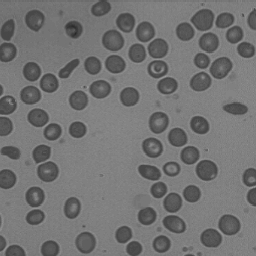
\includegraphics[width=5cm]{cells.png}} \hspace{1cm}
 \subfloat[Manual threshold.]{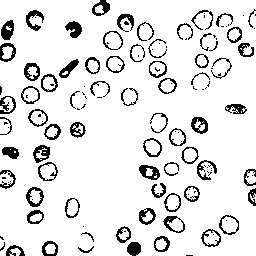
\includegraphics[width=5cm]{manual_threshold.png}}
 \caption{Simple thresholding.}
\end{figure}


\subsection{Grayscale image, $k=2$ in 1D}
The automatic threshold selection proposed can be coded as follows:
\begin{matlab}
function [s,B]=autothresh(A)
% Automatic threshold of image A
% return values:
%  s: threshold value
%  B: thresholded (binary) image

% initialization of s
s=0.5*(min(A(:)) + max(A(:)));
done = false;

% iterate until convergence of s
while ~done
    B=(A>=s);
    sNext=0.5*(mean(A(B))+mean(A(~B)));
    done=abs(s-sNext)<0.5; % convergence ?
    s=sNext;
end
\end{matlab}

Then, display the different results with:
\begin{matlab}
A=imread('cells.bmp');
% threshold determination
[s1,B]=autothresh(A);
s1

% Otsu (\matlabregistered{} function)
s2=graythresh(A);
s2=255*s2
C=(A>=s2);

% display results
figure;
subplot(2,2,1);imshow(A);title('Original image');
subplot(2,2,3);imshow(B);title('Automatic threshold');
subplot(2,2,4);imshow(C);title('Otsu threshold');
\end{matlab}

\begin{mwindow}
s1 =  104.0398
s2 =  105.5000
\end{mwindow}

\begin{figure}[htbp]
 \centering
 \subfloat[Proposed automatic method.]{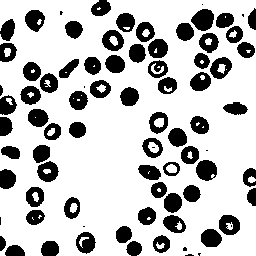
\includegraphics[width=5cm]{autothresh.png}}\hspace{1cm}
 \subfloat[Otsu method.]{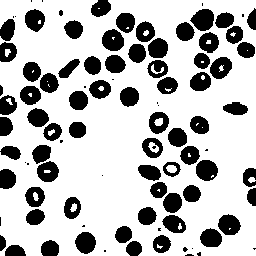
\includegraphics[width=5cm]{otsu.png}}
 \caption{}
\end{figure}


\subsection{Simulation example, $k=3$ in 2D}
The first function generates random points around a center. The objective is to retrieve the different clusters (aka classes). Depending on the distance and the distribution of the points, this could not yield to the expected result.
\begin{matlab}
function Y=generation(n, x, y)
% Generates n random points (normal law) around point
% of coordinates (x,y) 
Y = randn(n,2)+ones(n,2)*[x 0; 0 y];
\end{matlab}

\begin{matlab}
% Generate 3 point clouds
n=100;
X=[generation(n,3,4); generation(n,0,0); generation(n,-5,-3)];

% Classification
[idx, ctrs] = kmeans(X, 3, 'replicates', 5);

% Display results
figure();
plot(X(idx==1,1),X(idx==1,2),'r.','MarkerSize',12)
hold on
plot(X(idx==2,1),X(idx==2,2),'b+','MarkerSize',12)
plot(X(idx==3,1),X(idx==3,2),'g*','MarkerSize',12)

legend('Cluster 1','Cluster 2','Cluster 3')
\end{matlab}

\subsection{Color image segmentation by K-means: $k=3$ in 3D}
Each pixel of the color image is represented as a vector (3D point, with the RGB color values of the pixels). Then, the same method is performed. The result is represented in Fig.\ref{fig:tutorial:kmeans:matlab:color}.

\begin{matlab}
% Load image 
I=imread('Tv16.png');
I=double(I);
figure
imshow(I/255);

% Segmentation
nCouleurs = 3; % number of clusters
nLignes = size(I,1);
nCols   = size(I,2);

X = reshape(I, nLignes*nCols, 3);

[index centres] = kmeans(X, nCouleurs, 'distance', 'sqEuclidean', 'replicates', 3);

% 3D histogram (can be difficult to display, depending on machine)
id1=index==1;
id2=index==2;
id3=index==3;

figure
plot3(X(id1,1), X(id1,2), X(id1,3), 'r.')
hold on
plot3(X(id2,1), X(id2,2), X(id2,3), 'g.')
plot3(X(id3,1), X(id3,2), X(id3,3), 'b.')

% Label each pixel
labels = uint8(reshape(index, nLignes, nCols));
labels = imadjust(labels);

figure
subplot(121)
imshow(I/255);
subplot(122)
imshow(labels, []);
\end{matlab}

\begin{figure}[htbp]
\centering
\subfloat[Original image.]{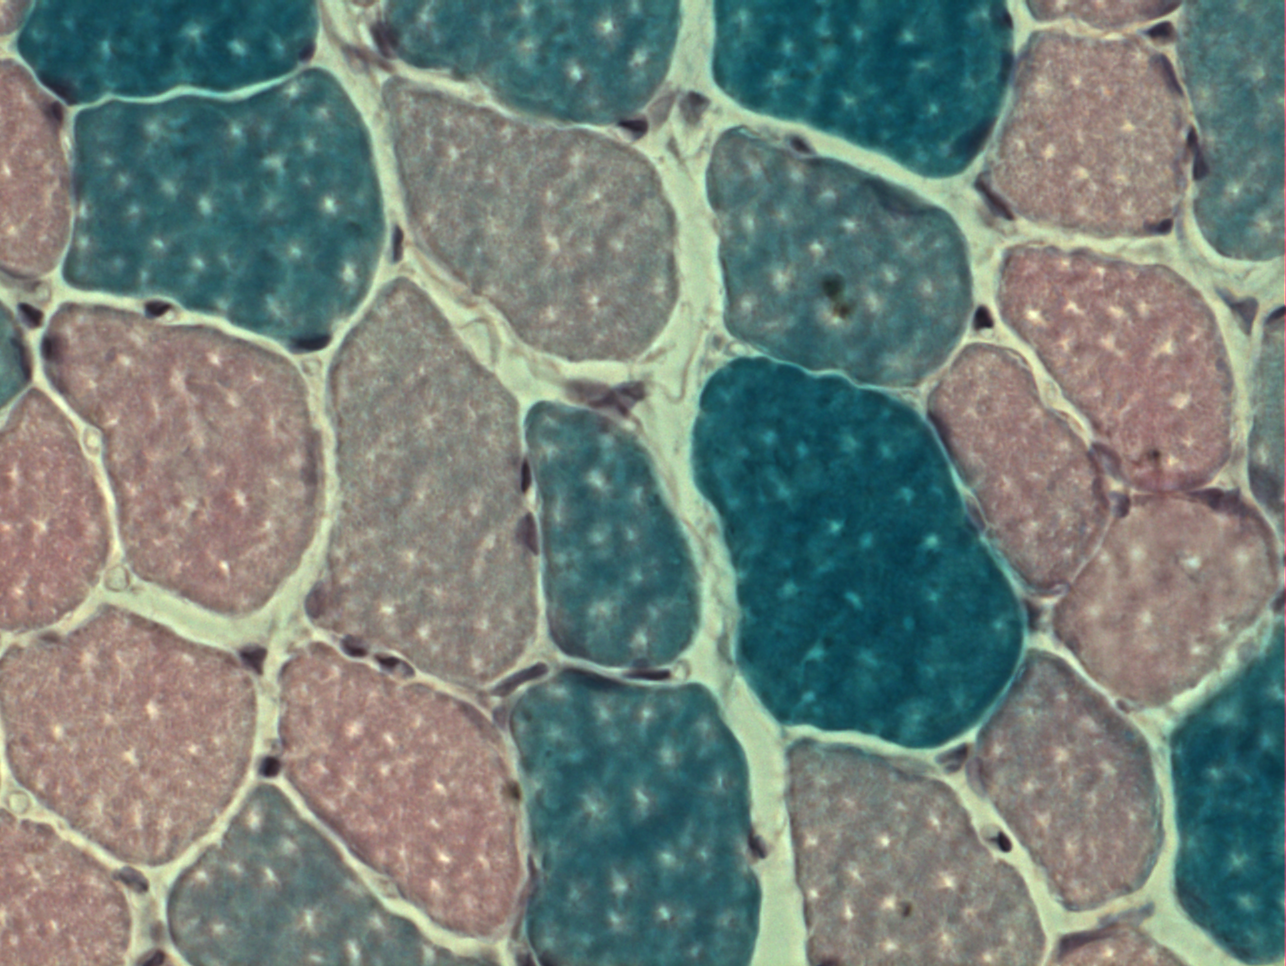
\includegraphics[width=5cm]{Tv16.png}}\hspace{1cm}
\subfloat[Segmented image.]{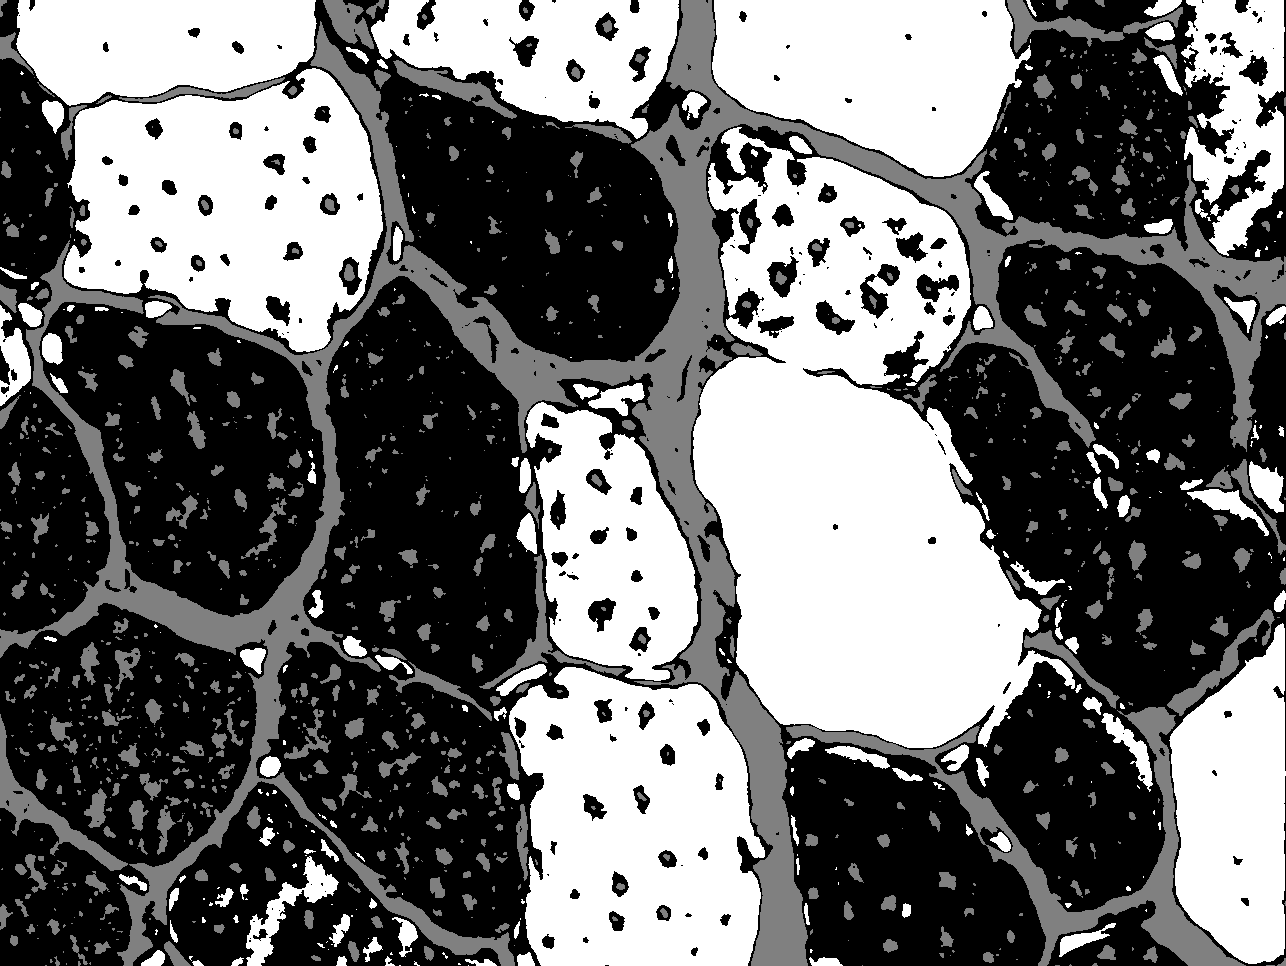
\includegraphics[width=5cm]{labels.png}}
\caption{K-means segmentation applied on a color image. The segmentation is applied in the color space. The spatial informations of the image structures is lost.}
\label{fig:tutorial:kmeans:matlab:color}
\end{figure}
